\documentclass{sigchi}

% Use this command to override the default ACM copyright statement (e.g. for preprints). 
% Consult the conference website for the camera-ready copyright statement.


%% EXAMPLE BEGIN -- HOW TO OVERRIDE THE DEFAULT COPYRIGHT STRIP -- (July 22, 2013 - Paul Baumann)
% \toappear{Permission to make digital or hard copies of all or part of this work for personal or classroom use is 	granted without fee provided that copies are not made or distributed for profit or commercial advantage and that copies bear this notice and the full citation on the first page. Copyrights for components of this work owned by others than ACM must be honored. Abstracting with credit is permitted. To copy otherwise, or republish, to post on servers or to redistribute to lists, requires prior specific permission and/or a fee. Request permissions from permissions@acm.org. \\
% {\emph{CHI'14}}, April 26--May 1, 2014, Toronto, Canada. \\
% Copyright \copyright~2014 ACM ISBN/14/04...\$15.00. \\
% DOI string from ACM form confirmation}
%% EXAMPLE END -- HOW TO OVERRIDE THE DEFAULT COPYRIGHT STRIP -- (July 22, 2013 - Paul Baumann)


% Arabic page numbers for submission. 
% Remove this line to eliminate page numbers for the camera ready copy
% \pagenumbering{arabic}


% Load basic packages
\usepackage{textcomp}
\usepackage{balance}  % to better equalize the last page
\usepackage{graphics} % for EPS, load graphicx instead
\usepackage{graphicx}  % include figures
\usepackage{times}    % comment if you want LaTeX's default font
\usepackage{url}      % llt: nicely formatted URLs

% llt: Define a global style for URLs, rather that the default one
\makeatletter
\def\url@leostyle{%
  \@ifundefined{selectfont}{\def\UrlFont{\sf}}{\def\UrlFont{\small\bf\ttfamily}}}
\makeatother
\urlstyle{leo}


% To make various LaTeX processors do the right thing with page size.
\def\pprw{8.5in}
\def\pprh{11in}
\special{papersize=\pprw,\pprh}
\setlength{\paperwidth}{\pprw}
\setlength{\paperheight}{\pprh}
\setlength{\pdfpagewidth}{\pprw}
\setlength{\pdfpageheight}{\pprh}

% Make sure hyperref comes last of your loaded packages, 
% to give it a fighting chance of not being over-written, 
% since its job is to redefine many LaTeX commands.
\usepackage[pdftex]{hyperref}
\hypersetup{
pdftitle={SIGCHI Conference Proceedings Format},
pdfauthor={LaTeX},
pdfkeywords={SIGCHI, proceedings, archival format},
bookmarksnumbered,
pdfstartview={FitH},
colorlinks,
citecolor=black,
filecolor=black,
linkcolor=black,
urlcolor=black,
breaklinks=true,
}

% create a shortcut to typeset table headings
\newcommand\tabhead[1]{\small\textbf{#1}}


% End of preamble. Here it comes the document.
\begin{document}

\title{Utilizing Weakly Trained GANs to produce 3D Models}

\numberofauthors{5}
\author{
  \alignauthor Kelechi M. Ikegwu\\
    \affaddr{Illinois Informatics Institute}\\
    \email{ikegwu2@illinois.edu}
  \alignauthor Hsuan-Yu Chen\\
    \affaddr{Department of Computer Science}\\
    \email{hychen2@illinois.edu}\\
  \alignauthor Ranjitha Kumar\\
    \affaddr{Department of Computer Science}\\
    \email{ jcao7@illinois.edu}\\
  \alignauthor Smit Desai\\
    \affaddr{School of Information Sciences}\\
    \email{smitad2@illinois.edu}\\
  \alignauthor Ranjitha Kumar\\
    \affaddr{Department of Computer Science}\\
    \email{ ranjitha@illinois.edu}\\  
}

%\author{
%  \alignauthor Kelechi M. Ikegwu\(^1\); Hsuan-Yu Chen\(^2\); Jiayi Cao\(^3\); Smit Desai\(^4\)\\
%    \affaddr{Illinois Informatics Institute\(^1\); Department of Computer Science\(^{2,3}\); School of Information Sciences\(^4\)}\\
%    \email{ikegwu2@illinois.edu\(^1\); hychen2@illinois.edu\(^2\); jcao7@illinois.edu\(^3\); smitad2@illinois.edu\(^4\)}\\
%  \alignauthor Ranjitha Kumar\\
%    \affaddr{Department of Computer Science}\\
%    \email{ ranjitha@illinois.edu}\\
%}

\maketitle

\begin{abstract}
Generative Adversarial Networks (GAN) have become the de-facto standard for generative models. However large amounts of data are required to achieve excellent performance which makes GANs challenging to apply to sparse datasets. In order to utilize GANs with sparse datasets we propose using weakly trained GANs to produce models which we then use to augment existing data. For this study we utilize 2 classes of a popular 3D dataset called 3DShapeNet to train on. Next data augmentation is performed on the original models using our proposed method, lastly we conduct a study to assess our models on Amazon Mechanical Turk.

\end{abstract}

\keywords{
	General Adversarial Networks; 3D-Models; Data Creation; Data Augmentation \newline
	%\textcolor{red}{Optional section to be included in your final version,  but strongly encouraged.}
}

\category{H.5.m.}{Information Interfaces and Presentation (e.g. HCI)}{Miscellaneous}
\category{I.2.m.}{Artificial Intelligence}{Miscellaneous}
\category{I.4.m.}{Image Processing and Computer Vision}{Miscellaneous}

\section{Introduction}

They \textquotesingle re a multitude of application areas where generative models are a promising method for solving certain problems. Generative Adversarial Networks (GAN) \cite{NIPS2014_5423} is a particular model  which is becoming the standard for generative models. However these models generally require a lot of data to generate sufficient results.

As an attempt to solve this problem we propose using the latent spaces from weakly trained GANs with sparse datasets to augment existing data. In the subsequent sections we frame our work with respect to research that has been conducted with GANs, we discuss about our methodology for performing transformations to our data, producing models, and performing an evaluation of our produced models.

\section{Related Works}

The foundation of this research is based on prior work of several key papers. We use a rich 3D model repository called ShapeNet \cite{shapenet2015} which contains a multitude of semantic categories organized under WordNet’s taxonomy \cite{Miller:1995:WLD:219717.219748}. In particular, we utilize the table and mug categories of ShapeNet. 


We used voxel models to efficiently deal with large amounts features from point cloud data. Similar methodology can be found in Daniel Maturana and Sebastian Scherer’s work in \cite{Maturana–2015–6018}, they propose VoxNet, an architecture by integrating a Volumetric Occupancy Grid representation with a supervised 3D Convolutional Neural Network (3D CNN). 

For our model we try to learn the probabilistic latent space of tables and chairs using Wu. J, Zhang. C, Xue. T, et. al’s work in \cite{3dgan}. All of the parameters are the same however, the generator \(G\) produces 32 x 32 x 32 object, our discriminator  \(D\) only accepts models with the size of 32 x 32 x 32,  the learning rate is .003.


\section{Methodology}
After obtaining the weakly trained models, we observe they possess some degree of orginal models’ characteristics but yet incomplete shape. The main issue is that most models have disconnected components and scattered voxel cubes in the 3D grid space due to the lack of training data. Therefore we undergo a series of morphology techniques to transform the models.

The first step was to extract the main component of the model by utilizing a depth-first search algorithm to get the largest connected component in the space.

After that, we notice there are holes in the surfaces of many models, therefore we used hole-filling algorithm to spot the holes and fix them. The algorithm used consists of invading the complementary of the shapes in input from the outer boundary of the image, using binary dilations. Holes are not connected to the boundary and are therefore not invaded. The result is the complementary subset of the invaded region.

We then take to-be-altered models from 3DShapeNet and apply a dilation algorithm to augment the models with the hole-filled weakly trained models as a space constraint. We will then obtain augmented tables with certain features from the weakly trained models.


\section{Generated Results}

Figure \ref{fig:table_results} shows examples of good results. We can see that the augmented part of model preserve some characteristics of the model. For example, some table’s have drawers or some other special design added to the table. However, there are also bad results where random voxel cubes are added to the original model (see Figure \ref{fig:bad_results}). 

We also performing image dilation using random noise to confirm that our GAN  is producing useful results (see Figure \ref{fig:table_random} ).

\begin{figure}
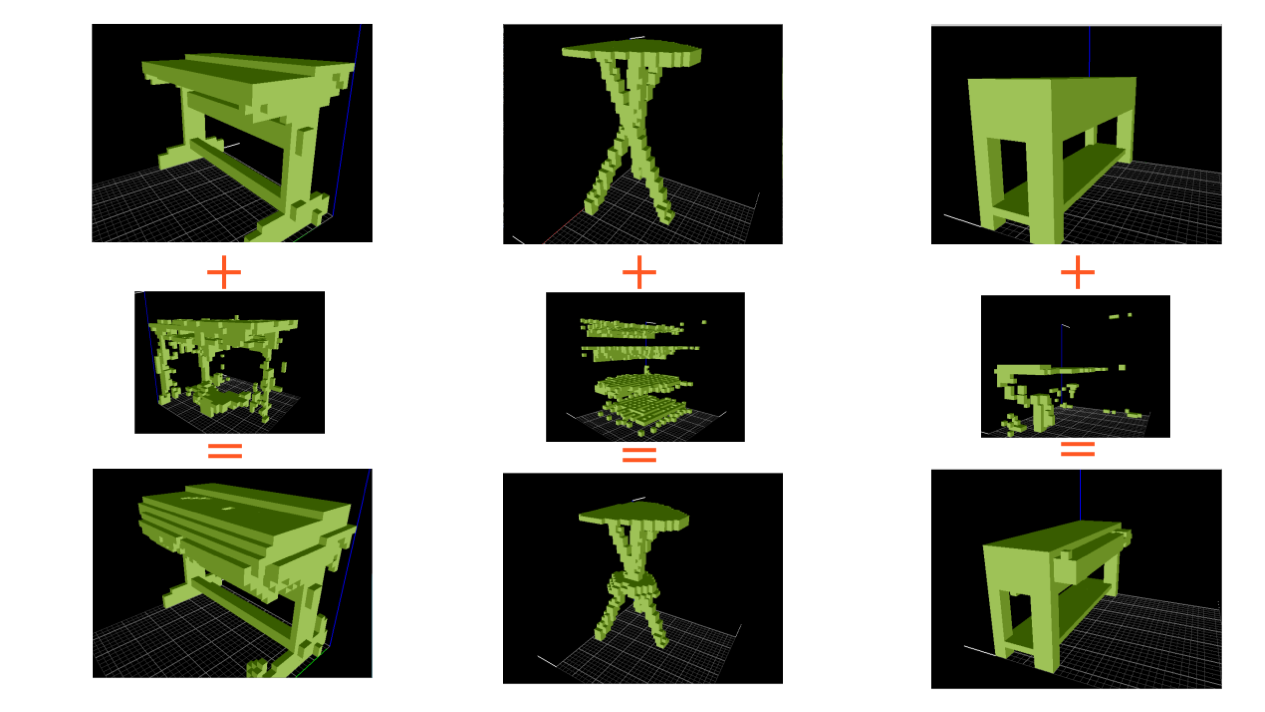
\includegraphics[width=0.4\textwidth]{figs/table_results.png}
\centering
\caption{The top row is the original table. Second row is the GAN produced model. The third row is our augmented table.}
\label{fig:table_results}
\end{figure}

\begin{figure}
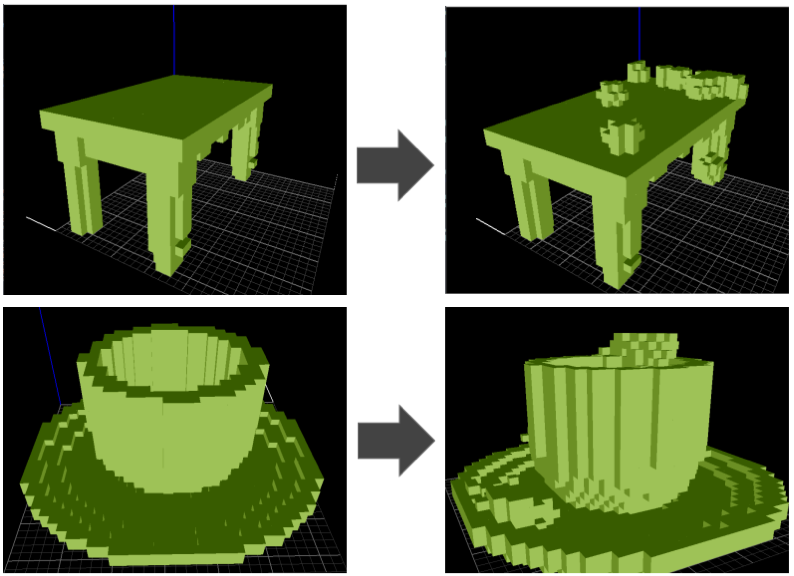
\includegraphics[width=0.3\textwidth]{figs/bad_results.png}
\centering
\caption{On the left is the original model. On the right is the poorly augmented model.}
\label{fig:bad_results}
\end{figure}

\begin{figure}
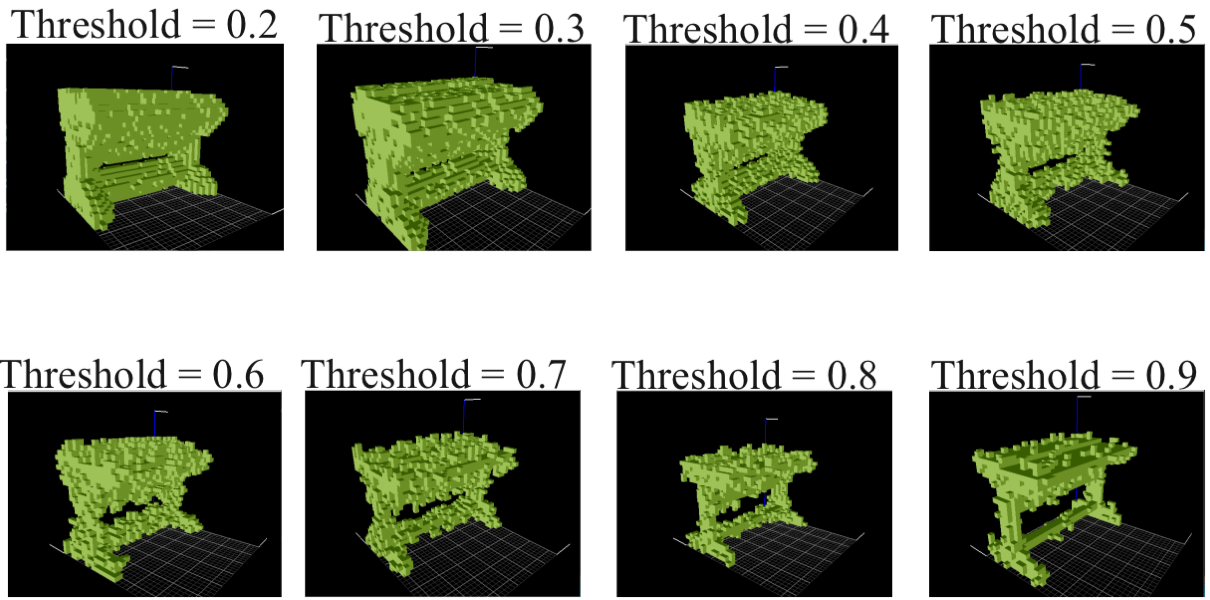
\includegraphics[width=0.4\textwidth]{figs/table_random.png}
\centering
\caption{We vary the probability of not adding additional random noise.}
\label{fig:table_random}
\end{figure}

\section{Evaluation}

One of the most important factors for determining how good the results are would be to find out how visually different the generated models are from the original models. For that purpose, we ran some tests on Amazon Mechanical Turk (AMT) where we asked users to rate the dissimilarity between the generated model and the original model on a 5 point Likert Scale. For the purpose of this experiment we chose to run our tests with tables as we believed that dissimilarities between tables would be easily discernible for the users. 
We recruited 30 workers for this experiment and we paid them \$0.05 per HIT. Three examples were provided to the workers for the sake of their understanding of the task. 
On an average, the workers rated the dissimilarity between the generated and the original model as 3.2 (fairly significant). Along with that 27/30 workers perceived the tables to be practically usable. 



\section{Conclusion \& Future Work}
To summarize we propose a method for performing data augmentation with 3D voxelized models. We utilized 2 classes from ShapeNet with a sparse number of examples. We then perform an evaluation on AMT.

In the future we plan to explore more sophisticated techniques for generating more data. For example we plan to explore morphing models directly from ShapeNet. 

In addition to this we plan to share the results of training on our generated models to determine if our model learned the latent space better than the model that trained on ~10K examples from ShapeNet. We also plan to perform a comparative analysis against a GAN that trains with data from sophisticated morphing techniques and another GAN that used our augmented data from our methodology.


\section{Acknowledgments}
We'd like to thank Dr. Ranjitha Kumar for supplying us with necessary resources to train our models and also for her advice and mentorship.
\balance


\bibliographystyle{acm-sigchi}
\bibliography{CS598RK-g7-sp17}
\end{document}
